We now return to the setting of training models to in-context learn linear functions and explore different factors that lead to successful in-context learning.

\paragraph{Problem Dimension and Capacity.}
In Section \ref{sec:linear_functions} and \ref{sec:distribution_shifts}, we saw that Transformer models can be trained to in-context learn 20-dimensional linear functions accurately and relatively robustly. 
To explore the interplay between problem dimensionality and capacity, we also consider models with fewer parameters (see Appendix~\ref{app:architecture}) and train each architecture on \{10, 30, 40, 50\}-dimensional problems.
In Figure~\ref{fig:capacity}, we plot the model error with $2d$ in-context examples as we vary the problem dimension $d$ and the model capacity. 
In the standard setting, i.e., when the training and inference time prompt distributions are the same, we observe that the  error decreases as we increase the capacity or reduce the problem dimensionality (see Figure~\ref{fig:cap_standard}). 
Thus, model capacity helps perform accurate in-context learning.
For out-of-distribution prompts, we observe that the settings where the input covariance is skewed or where in-context example inputs and query inputs lie in different orthants are particularly challenging, especially for higher dimensional problems.
However, the error decreases considerably (in most cases) as we increase the model capacity, even when absolute decrease in the standard error is small (see Figure \ref{fig:cap_random} and \ref{fig:cap_skewed}). 
See Appendix \ref{app:capacity}  for additional plots.



\begin{figure}[htp]
    \hfill
    \begin{subfigure}[b]{0.28\textwidth}
        \centering
        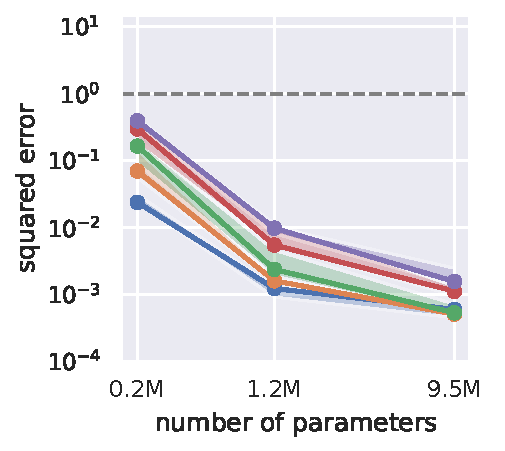
\includegraphics[height=.9\textwidth]{figures/capacity_standard.pdf}
        \caption{Standard}
        \label{fig:cap_standard}
    \end{subfigure}
    \hfill
    \begin{subfigure}[b]{0.28\textwidth}
        \centering
        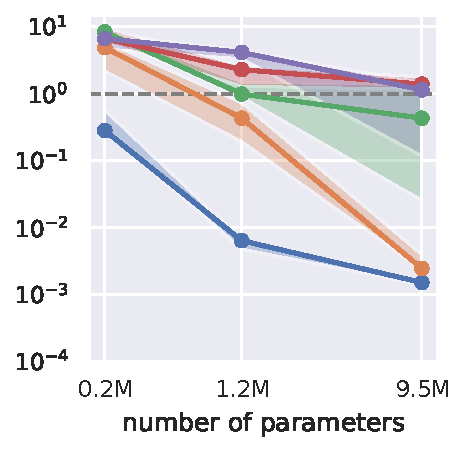
\includegraphics[height=.9\textwidth]{figures/capacity_random.pdf}
        \caption{Different orthants}
        \label{fig:cap_random}
    \end{subfigure}
    \hfill
    \begin{subfigure}[b]{0.28\textwidth}
        \centering
        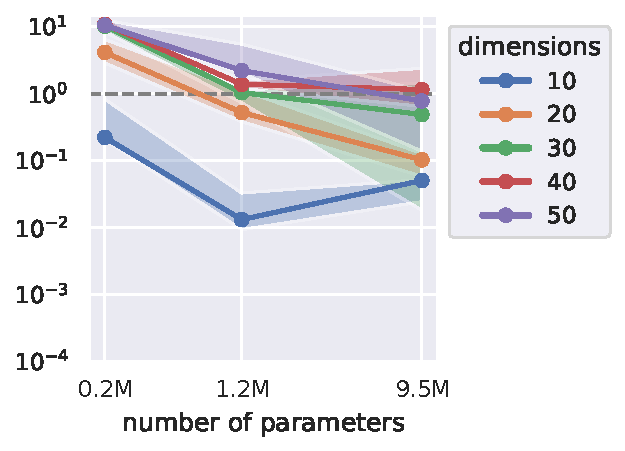
\includegraphics[height=.9\textwidth]{figures/capacity_skewed.pdf}
        \caption{Skewed covariance}
        \label{fig:cap_skewed}
    \end{subfigure}
    \hfill
    \phantom{dsada}
    \caption{\emph{Understanding the effect of model capacity and problem dimension on in-context learning performance for in-distribution (a) and out-of-distribution (b,c) prompts.} We train Transformers to in-context learn linear functions and plot the error with $2d$ in-context examples as we vary problem dimension $d$ and model capacity.  Capacity helps with in-context learning in most cases, especially on out-of-distribution prompts (even when the absolute gains in the in-distribution setting are small). We train 3 models in each case with different random seeds, and show the median error (solid lines), and the minimum and maximum errors (shaded region). (See Appendix~\ref{app:variance} for training variance analysis.)}
    \label{fig:capacity}
\end{figure}


\paragraph{Curriculum.}
We train our models using curriculum learning. That is, we initially draw the prompt inputs from a fixed $5$ dimensional subspace (by setting some of the coordinates to $0$) with prompt length $11$ (number of input-output pairs), and increase the subspace dimension by $1$ and prompt length by $2$ every $2,000$ training steps, until the subspace dimension reaches the ambient dimension $d$ and prompt length reaches $2d+1$ (see Appendix \ref{app:training} for details).
This process can also be viewed as gradually increasing the complexity of the function class.
This speeds up training drastically, especially for higher dimensional problems: for dimension 50, the loss barely decreases through the 500k training steps without curriculum but reaches close to the optimum with curriculum. 
For the 20 dimensional problem where we were able to train the model without curriculum within the training (step count) budget, we did not observe any qualitative difference in accuracy or robustness compared to the model trained with curriculum. 
We include plots comparing the speed and accuracy of training with and without curriculum in Appendix \ref{app:curriculum}.

Notably, when training Transformers without curriculum, there is an initial---relatively long---period  in training where the loss does not decrease, followed by a period of sharp decrease.
The length of this period varies with training randomness and seems to increase on average with problem dimension.
Understanding the model just before and after this transition moment is a promising future direction, which can give insights into the emergence of  in-context learning. 
Interestingly,~\citet{olsson2022context} observe a similar jump in the in-context learning ability of a language model which they attribute to the formation of ``induction heads''.

\paragraph{Number of distinct prompts or functions seen during training.} 
To estimate the amount of training data required for in-context learning, we perform two ablation studies. In the first study, we limit the number of distinct prompts seen during training. That is, we create a set of $n_p$ randomly generated prompts (as described in Section~\ref{sec:setting}), and sample prompts from this set during training (here, we train without curriculum, as it would introduce additional prompts during the warmup phase). In the second study, we only limit the number of distinct functions used for training.
That is we create a set of $n_w$ randomly chosen vectors (corresponding to $n_w$ linear functions) and sample weight vectors uniformly from that set to generate the training prompts (the inputs are still sampled from $N(0, I_d)$ for each training prompt).
We find that the amount of training data required is relatively small: non-trivial in-context learning is possible with $n_p = 100\text{k}$  or $n_w = 1\text{k}$, and the error drops close to that of the unrestricted model (discussed in Section \ref{sec:linear_functions}) with $n_p = 1\text{M}$ or $n_w = 10\text{k}$ (details in Appendix \ref{app:distinct_funcs}).
For context, in Section \ref{sec:linear_functions}, the model is trained on fresh prompts each step, thus encountering 32M distinct functions and prompts (500k training steps with 64 prompts/batch). 
%As discussed in Section \ref{sec:linear_functions_1}, these results suggest that the trained models are not performing in-context learning by memorizing the training prompts or weight vectors used to generate them, as that would lead to a much higher error.